\appendix
%% Правка оформления ссылок на приложения:
%http://tex.stackexchange.com/questions/56839/chaptername-is-used-even-for-appendix-chapters-in-toc
%http://tex.stackexchange.com/questions/59349/table-of-contents-with-chapter-and-appendix
%% требует двойной компиляции
\addtocontents{toc}{\def\protect\cftchappresnum{\MakeUppercase{\appendixname{}} }%
\setlength{\cftchapnumwidth}{\widthof{\cftchapfont\MakeUppercase{\appendixname~Б}\cftchapaftersnum}}%
}
%% Оформление заголовков приложений ближе к ГОСТ:
\sectionformat{\chapter}[display]{% Параметры заголовков разделов в тексте
    label=\MakeUppercase{\appendixname}\ \thechapter,% (ГОСТ Р 2.105, 4.3.6)
    labelsep=20pt,
}
%%\renewcommand{\chaptername}{ПРИЛОЖЕНИЕ}
\renewcommand\thechapter{\Asbuk{chapter}} % Чтобы приложения русскими буквами нумеровались
\begin{landscape}
\chapter{АППРОКСИМАЦИИ ФУНКЦИИ MOS ДЛЯ ПЕРЕДАЧИ ВИДЕОДАННЫХ}
\label{AppA}
   \begin{longtable}[H]{| C{10cm} | C{13cm} | C{2cm} |}
    \caption{Аппроксимации функции MOS для передачи видеоданных}\label{tab:appraximations} \\
    \hline
    Формула & Описание & Источник \\
    \hline
    \multicolumn{3}{|c|}{Процент замирания воспроизведения потока (Stalling, Rebuffering Percentage)}\\
    \hline
    ${{g}_{i}}=\underset{t~\to \infty }{\mathop{\lim }}\,\frac{r{{b}_{i}}\left( t \right)}{r{{b}_{i}}\left( t \right)+{{d}_{i}}\left( t \right)}$\newline
$Minimize:\underset{i}{\mathop \sum }\,{{g}_{i}}$  & $g_i$~--~процент времени, когда пользователь наблюдал прерывание воспроизведения потока; \newline $rb_i(t)$~--~длительность замираний воспроизведения потока за время $t$; \newline $d_i(t)$~--~длительность просмотренной последовательности за время $t$. & \cite{QoE_Ozgur,past_tur}\\
    \hline
    ${{q}_{i}}=\underset{t~\to \infty }{\mathop{\text{lim}}}\,\frac{{{w}_{i}}\left( t \right)}{{{d}_{i}}\left( t \right)}$ \newline
$Minimize:\underset{i}{\mathop \sum }\,{{q}_{i}}$  & $w_i(t)$~--~длительность ожидания в течении времени t, учитывающее начальные буферизации и прерывания воспроизведения потока. & \cite{Bakin_Globecom}\\
    \hline
    \multicolumn{3}{|c|}{Взвешенные суммы характеристик воспроизведения}\\
    \hline
    $MO{{S}_{i}}={{f}_{RATE}}\left( {{R}_{i}} \right)$\newline $Maximize:\sum\limits_{i}{MO{{S}_{i}}}$ & $R_i(t)$~--~битовая скорость просматриваемого потока. & \cite{Essaili_Rate} \\
    \hline
    ${{f}_{i}}=~{{k}_{1}}\ln {{R}_{i}}-{{k}_{2}}\frac{r{{b}_{i}}\left( t \right)}{{{d}_{i}}\left( t \right)}$\newline $Maximize:\underset{i}{\mathop \sum }\,{{f}_{i}}$ & $R_i(t)$~--~битовая скорость просматриваемого потока;\newline $k_1,k_2$~--~весовые коэффициенты приоритета функции от битовой скорости и замираний воспроизведения соответственно, причем $k_1 << k_2$. & \cite{Suai2015} \\
    \hline
    $Minimize:W\lambda -~\theta ~$ & $\lambda$~--~средний процент времени прерывания воспроизведения по всем пользователям;\newline $\theta$~--~среднее значение скорости битовой репрезентации по всем пользователям; \newline $W$~--~весовой коэффициент приоритета прерывания воспроизведения, сравним со значением $\theta$.& \cite{7179392} \\
    \hline
    $Qo{{E}_{i}}\left[ t \right]={{W}_{1}}$\newline$\log ({{R}_{i}}\left[ t \right]~-{{W}_{2}}{{\left( Bu{{f}_{i}}\left[ t \right]-Bu{{f}_{thr}} \right)}^{2}}$\newline$-{{W}_{3}}{{\left( {{R}_{i}}\left[ t \right]-{{R}_{i}}\left[ t-1 \right] \right)}^{2}})$ \newline $Maximize:\underset{i}{\mathop \sum }\,Qo{{E}_{i}}\left[ t \right]$ & $W_1, W_2,W_3$~--~весовые коэффициенты;\newline $R_i[t]$~--~битовая скорость в момент времени $t$;\newline $Buf_i[t]$~--~уровень буфера в момент времени $t$;\newline $Buf_{thr}$~--~ пороговое значение уровня буфера. & \cite{widash}  \\
    \hline
    $MO{{S}_{i}}=\frac{{{a}_{1}}+{{a}_{2}}Fr{{R}_{i}}+{{a}_{3}}\log \left( R_{i}^{TCP} \right)}{1+{{a}_{4}}P{{L}_{i}}+{{a}_{5}}{{\left( P{{L}_{i}} \right)}^{2}}}$\newline$Maximize:\sum\limits_{i}{MO{{S}_{i}}}$ & $a_j$~--~коэффициенты, зависящие от характеристик просматриваемого контента;\newline $FrR_i$~--~частота кадров потока; $R_{i}^{TCP}$~--~скорость получения информации;\newline $P{{L}_{i}}$~--~вероятность потери пакета. & \cite{5508802} \\
    \hline
    $MO{{S}_{i}}=\frac{b-a}{1+{{c}_{0}}{{\left( R_{i}^{TCP} \right)}^{-c1}}{{\left( {{c}_{2}} \right)}^{SU{{D}_{i}}}}}+a$\newline$Maximize:\underset{i}{\mathop \sum }\,MO{{S}_{i}}$ & $a,b$~--~нормирующие константы;\newline $c_j$~--~константы, подобранные в ходе эксперимента;\newline $SU{{D}_{i}}$~--~длительность ожидания начала воспроизведения. & \cite{6825149,6883466} \\
    \hline
    $\left\{ \begin{matrix}
   MO{{S}_{Res}}\left( Res{{l}_{i}} \right)=1.475\log \left( Res{{l}_{i}} \right)-6.15  \\
   MO{{S}_{Reb}}\left( RebRat{{e}_{i}} \right)=0.738~{{e}^{-RebRat{{e}_{i}}}}  \\
   MO{{S}_{SUD}}\left( SU{{D}_{i}} \right)=-0.02~SU{{D}_{i}}+2.53  \\
\end{matrix} \right.$\newline$MO{{S}_{i}}=0.174~MO{{S}_{Res}}\left( Res{{l}_{i}} \right)MO{{S}_{Reb}}{{\left( RebRate \right)}_{i}}\cdot$\newline$\cdot MO{{S}_{SUD}}\left( SU{{D}_{i}} \right)$\newline$Maximize:\sum\limits_{i}{MO{{S}_{i}}}$ & $Res{{l}_{i}}$~--~разрешение репрезентации;\newline$RebRate_i$~--~отношение времени просмотра к длительности опустошения буфера. & \cite{Chen_Chang_Wei} \\
    \hline

\end{longtable}
\end{landscape}
\chapter{ПАРАМЕТРЫ МОДЕЛИРОВАНИЯ}
\label{AppB}

\begin{longtable}[H]{| C{10cm} | C{7cm} |}
    \caption{Параметры моделирования}\label{tab:SimParams} \\
		\hline
 		\textbf{Название параметра} & \textbf{Значение} \\
 		\hline
 		\multicolumn{2}{|c|}{\textbf{Общие положения}} \\
		\hline
		Максимальная удаленность пользователей от базовой станции $X_{max}$ & 700 м \\
		\hline
		Типы трафика & Только видео \\
		\hline
		Длительность моделирования & 360000 с \\
		\hline
		Длительность интервала планирования & 1 мс \\
		\hline

		\multicolumn{2}{|c|}{\textbf{Беспроводной канал}} \\
		\hline
		Модель затухания распространения сигнала & Окамура-Хата \\
		\hline
		Окружение & Городская застройка \\
		\hline
		Тип города & Большой город \\
		\hline
		Мощность передатчика базовой станции & 44 дБм \\
		\hline
		Мощность передатчика пользовательского устройства & 23 дБм \\
		\hline
		Коэффициент усиления антенны базовой станции и пользовательского устройства & 10 дБ \\
		\hline
		Несущая частота & 2 ГГц \\
		\hline
		Ширина полосы передачи & 10 МГц \\
		\hline
		Модель ошибки при передаче данных & Отсутствует \\
		\hline

		\multicolumn{2}{|c|}{\textbf{Плоские замирания}} \\
		\hline
		Модель & Extended Pedestrian A (EPA) \\
		\hline
		Движение окружения  & 3 км/ч \\
		\hline
		Длительность генерируемой последовательности & 10 с \\
		\hline
		Несущая частота & 2 ГГц \\
		\hline

		\multicolumn{2}{|c|}{\textbf{TCP протокол}} \\
		\hline
		Стандарт & TCP NewReno \\
		\hline
		Размер фрагментации пакета  & 1440 Б \\
		\hline
		Минимальное значения таймаута & 1 с \\
		\hline
		Начальный размер окна  & 4320 Б \\
		\hline
		Ограничение начального роста окна быстрого старта & Неограничен \\
		\hline
		Размер буфера на приемной и передающей стороне  & 6 МБ \\
		\hline

		\multicolumn{2}{|c|}{\textbf{Алгоритм планирования для неадаптивных видеопотоков}} \\
		\hline
		Интервал усреднения оценки скорости передачи информации ($\bar{w}_{S}$) & 1000 мс \\
		\hline
		Интервал усреднения оценки максимальной пропускной способности канала ($\bar{w}_{C}$) & 1000 мс \\
		\hline
		Минимальная гарантированная скорость получения информации ($S^{min}$) & 100 Кб/с \\
		\hline

		\multicolumn{2}{|c|}{\textbf{Видео контент}} \\
		\hline
		Длительность видео & 300 с \\
		\hline
		Битовые скорости потока неадаптивных видеопоследовательностей & 1 Мбит/с \\
		\hline
		Битовые скорости потока адаптивных видеопоследовательностей & [1, 4.5] Мбит/с \\
		\hline

		\multicolumn{2}{|c|}{\textbf{Видеоплеер}} \\
		\hline
		Длительность сегмента видеоданных & 2 с \\
		\hline
		Размер начальной буферизации & 4 с \\
		\hline
		Максимальный размер буфера & 10 с \\
		\hline
		Адаптация видеопотока & Соответствует параметрам, представленным в таблице \ref{tab:DashJSParams} \\
		\hline

		\multicolumn{2}{|c|}{\textbf{Поведение пользователя}} \\
		\hline
		Начальная задержка при заказе видео & Равномерная случайная величина в отрезке [1, 60] с \\
		\hline
		Пауза между просмотрами видео & Усеченная экспоненциальная случайная величина в отрезке [15, 45] с со средним значением 30 с\\
		\hline
\end{longtable}
\begin{landscape}
\chapter{ГРАФИЧЕСКОЕ ПРЕДСТАВЛЕНИЕ ЗАВИСИМОСТЕЙ РАЗДЕЛОВ}
\label{AppС}
\begin{figure}[H]
\begin{center}
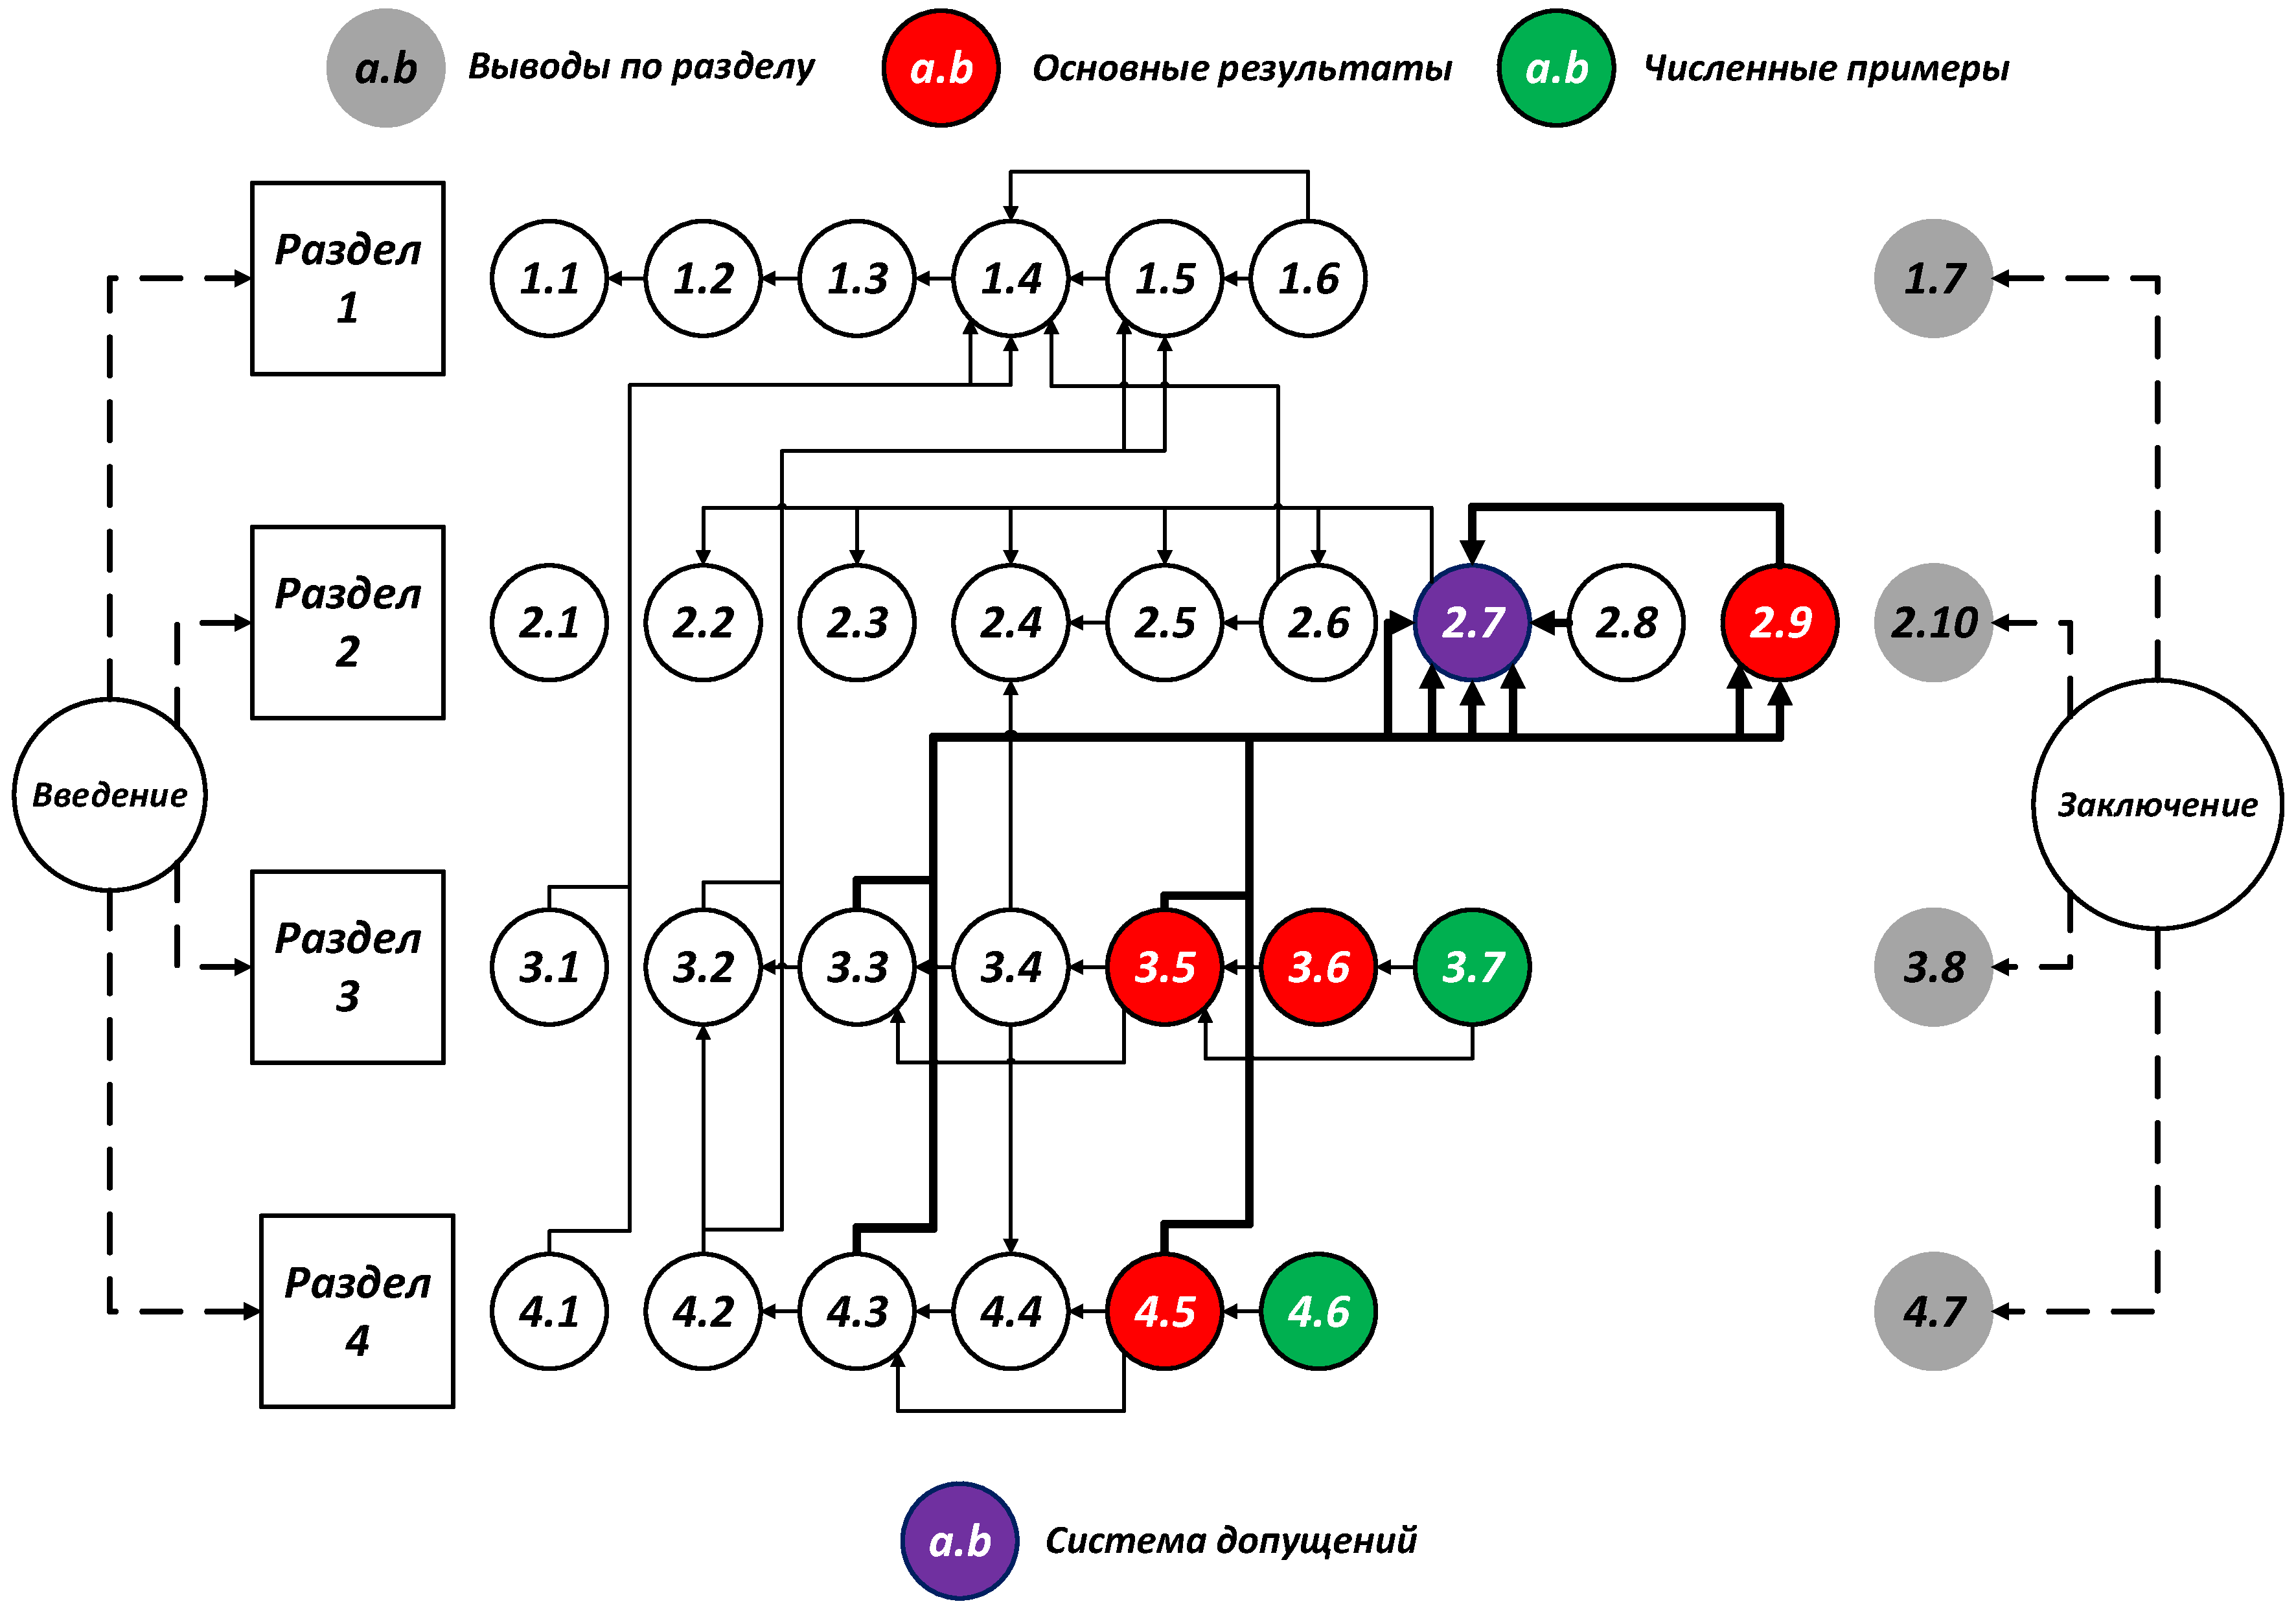
\includegraphics[width=1.2\textwidth,height=0.7\textheight]{graph_horizontal.pdf}
\caption{Графическое представление зависимостей подразделов в диссертационном исследовании}
\label{fig:graph_horizontal.pdf}
\end{center}
\end{figure}
\end{landscape}
\chapter{АКТЫ О ВНЕДРЕНИИ}
\label{AppD}
\begin{center}
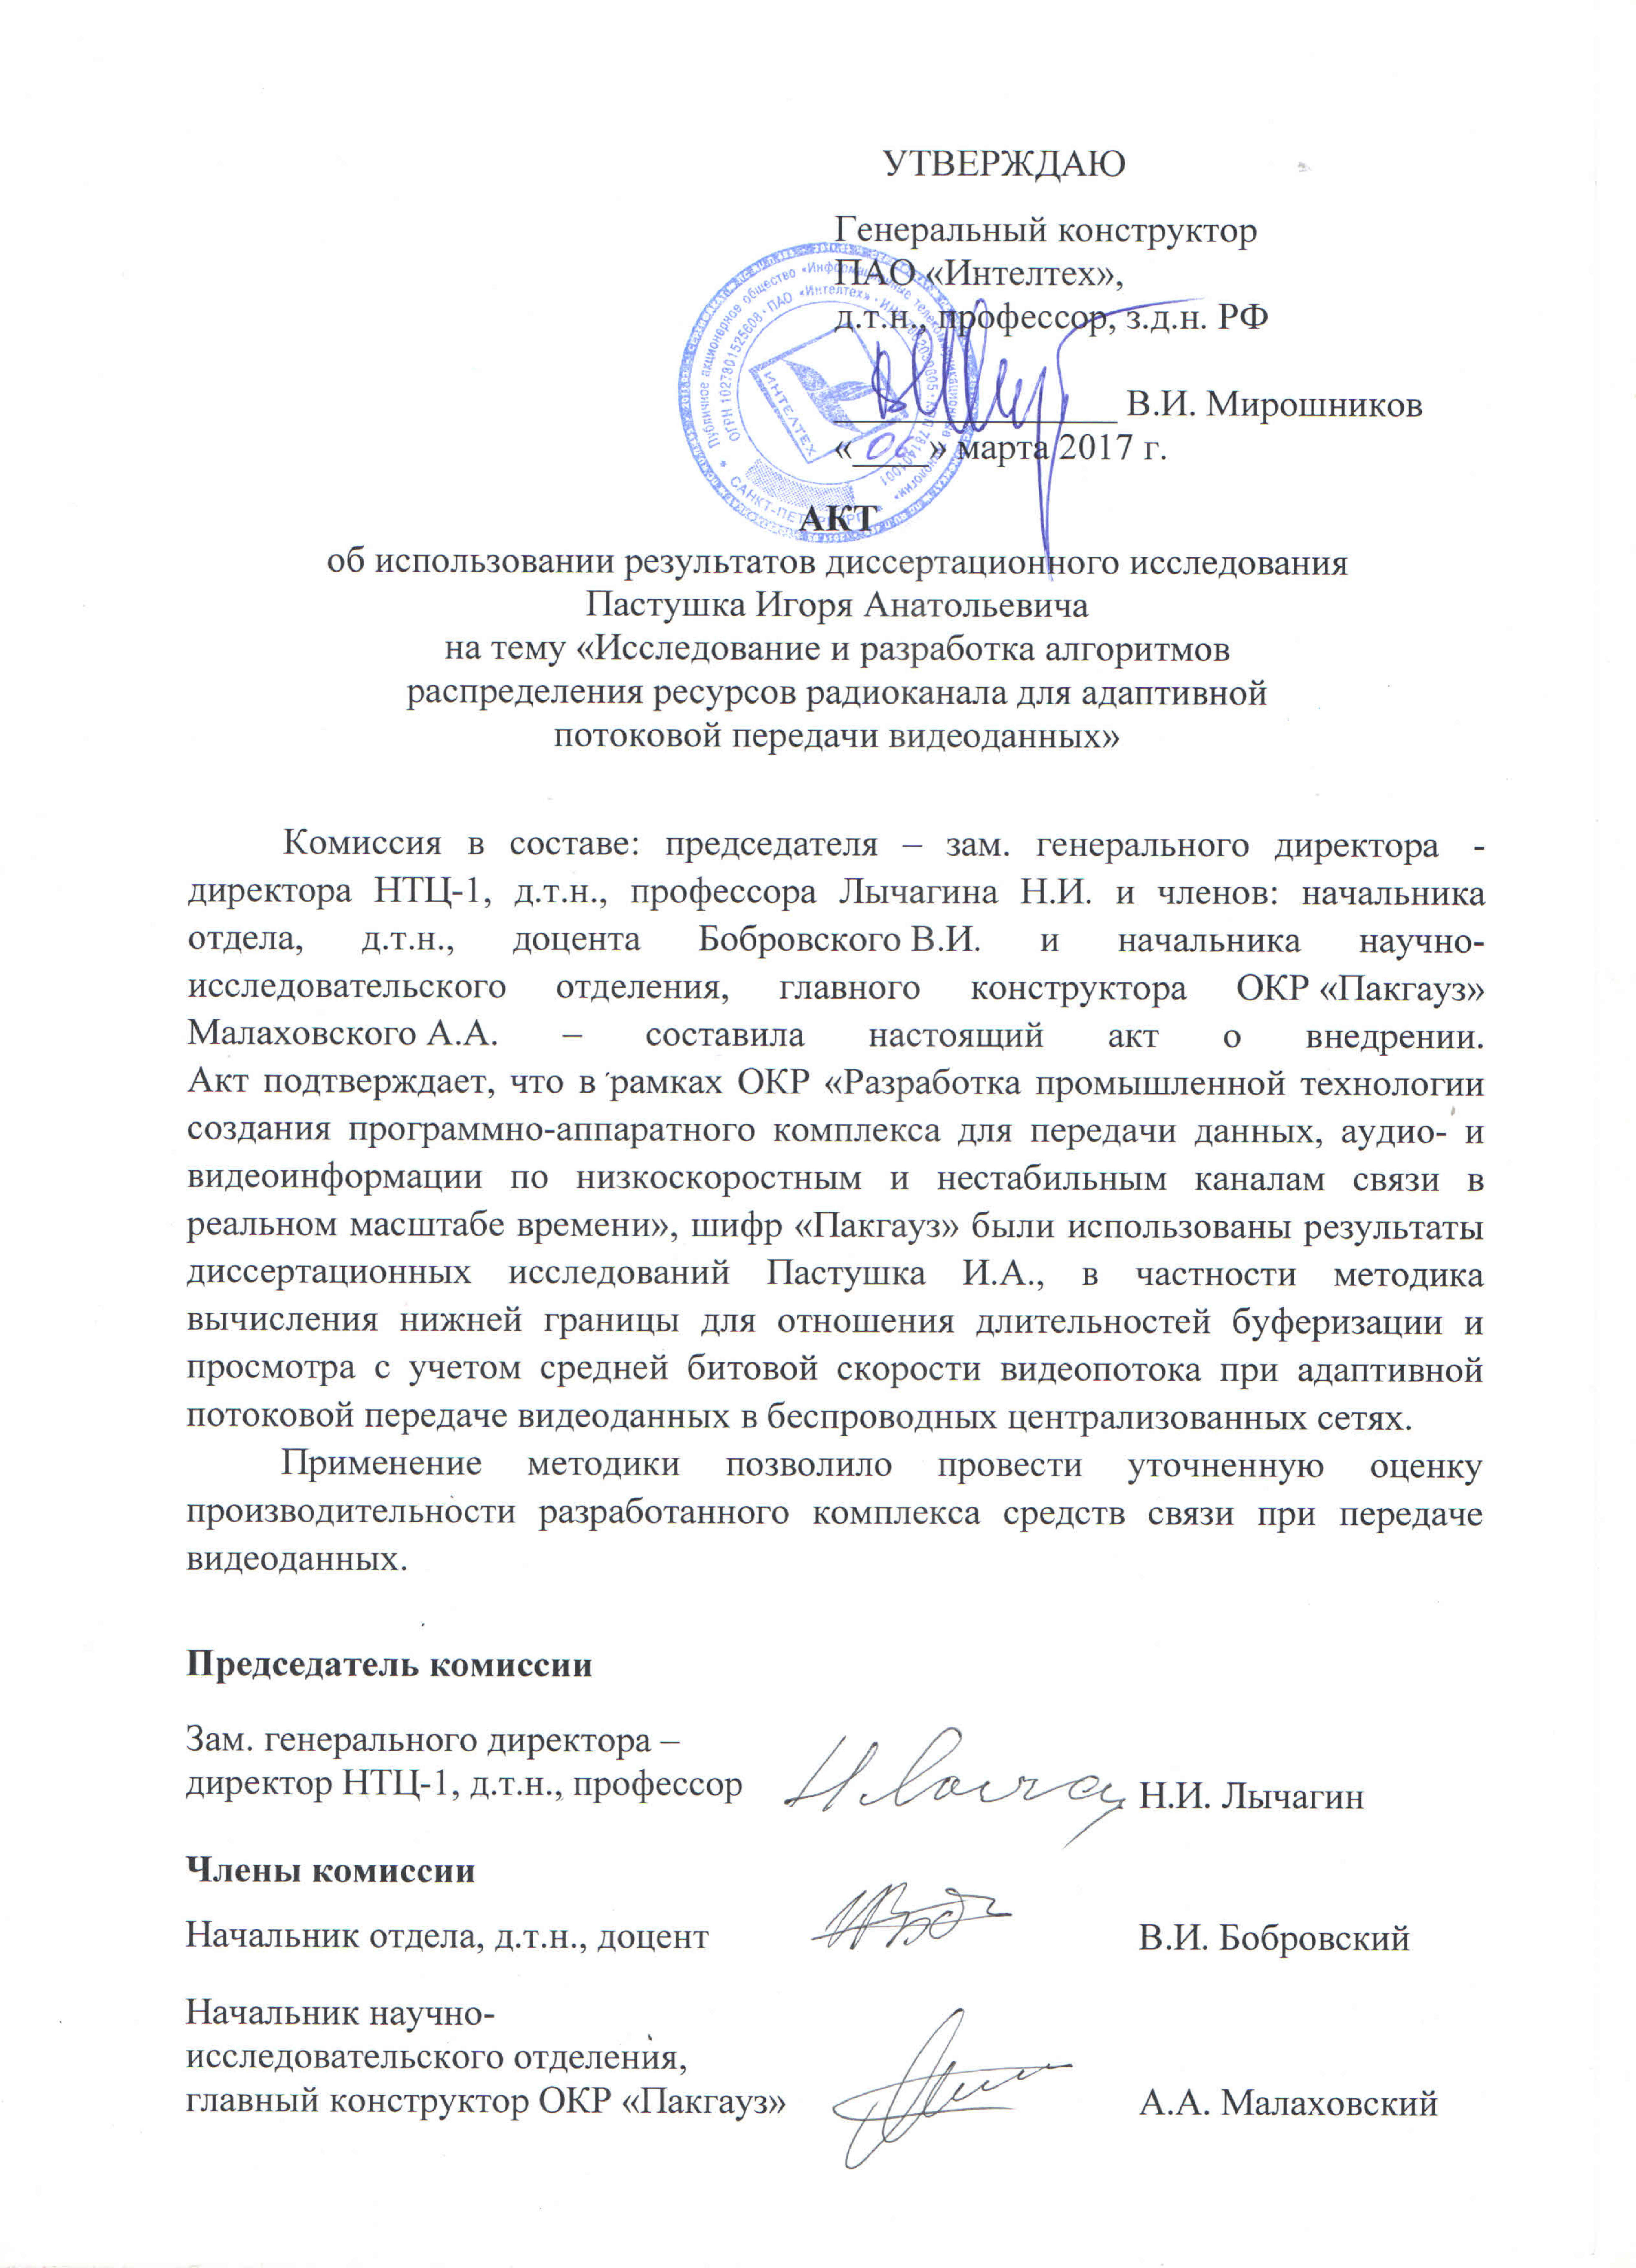
\includegraphics[width=1\textwidth,height=0.8\textheight]{appendix/Inteltech.pdf}
\end{center}
%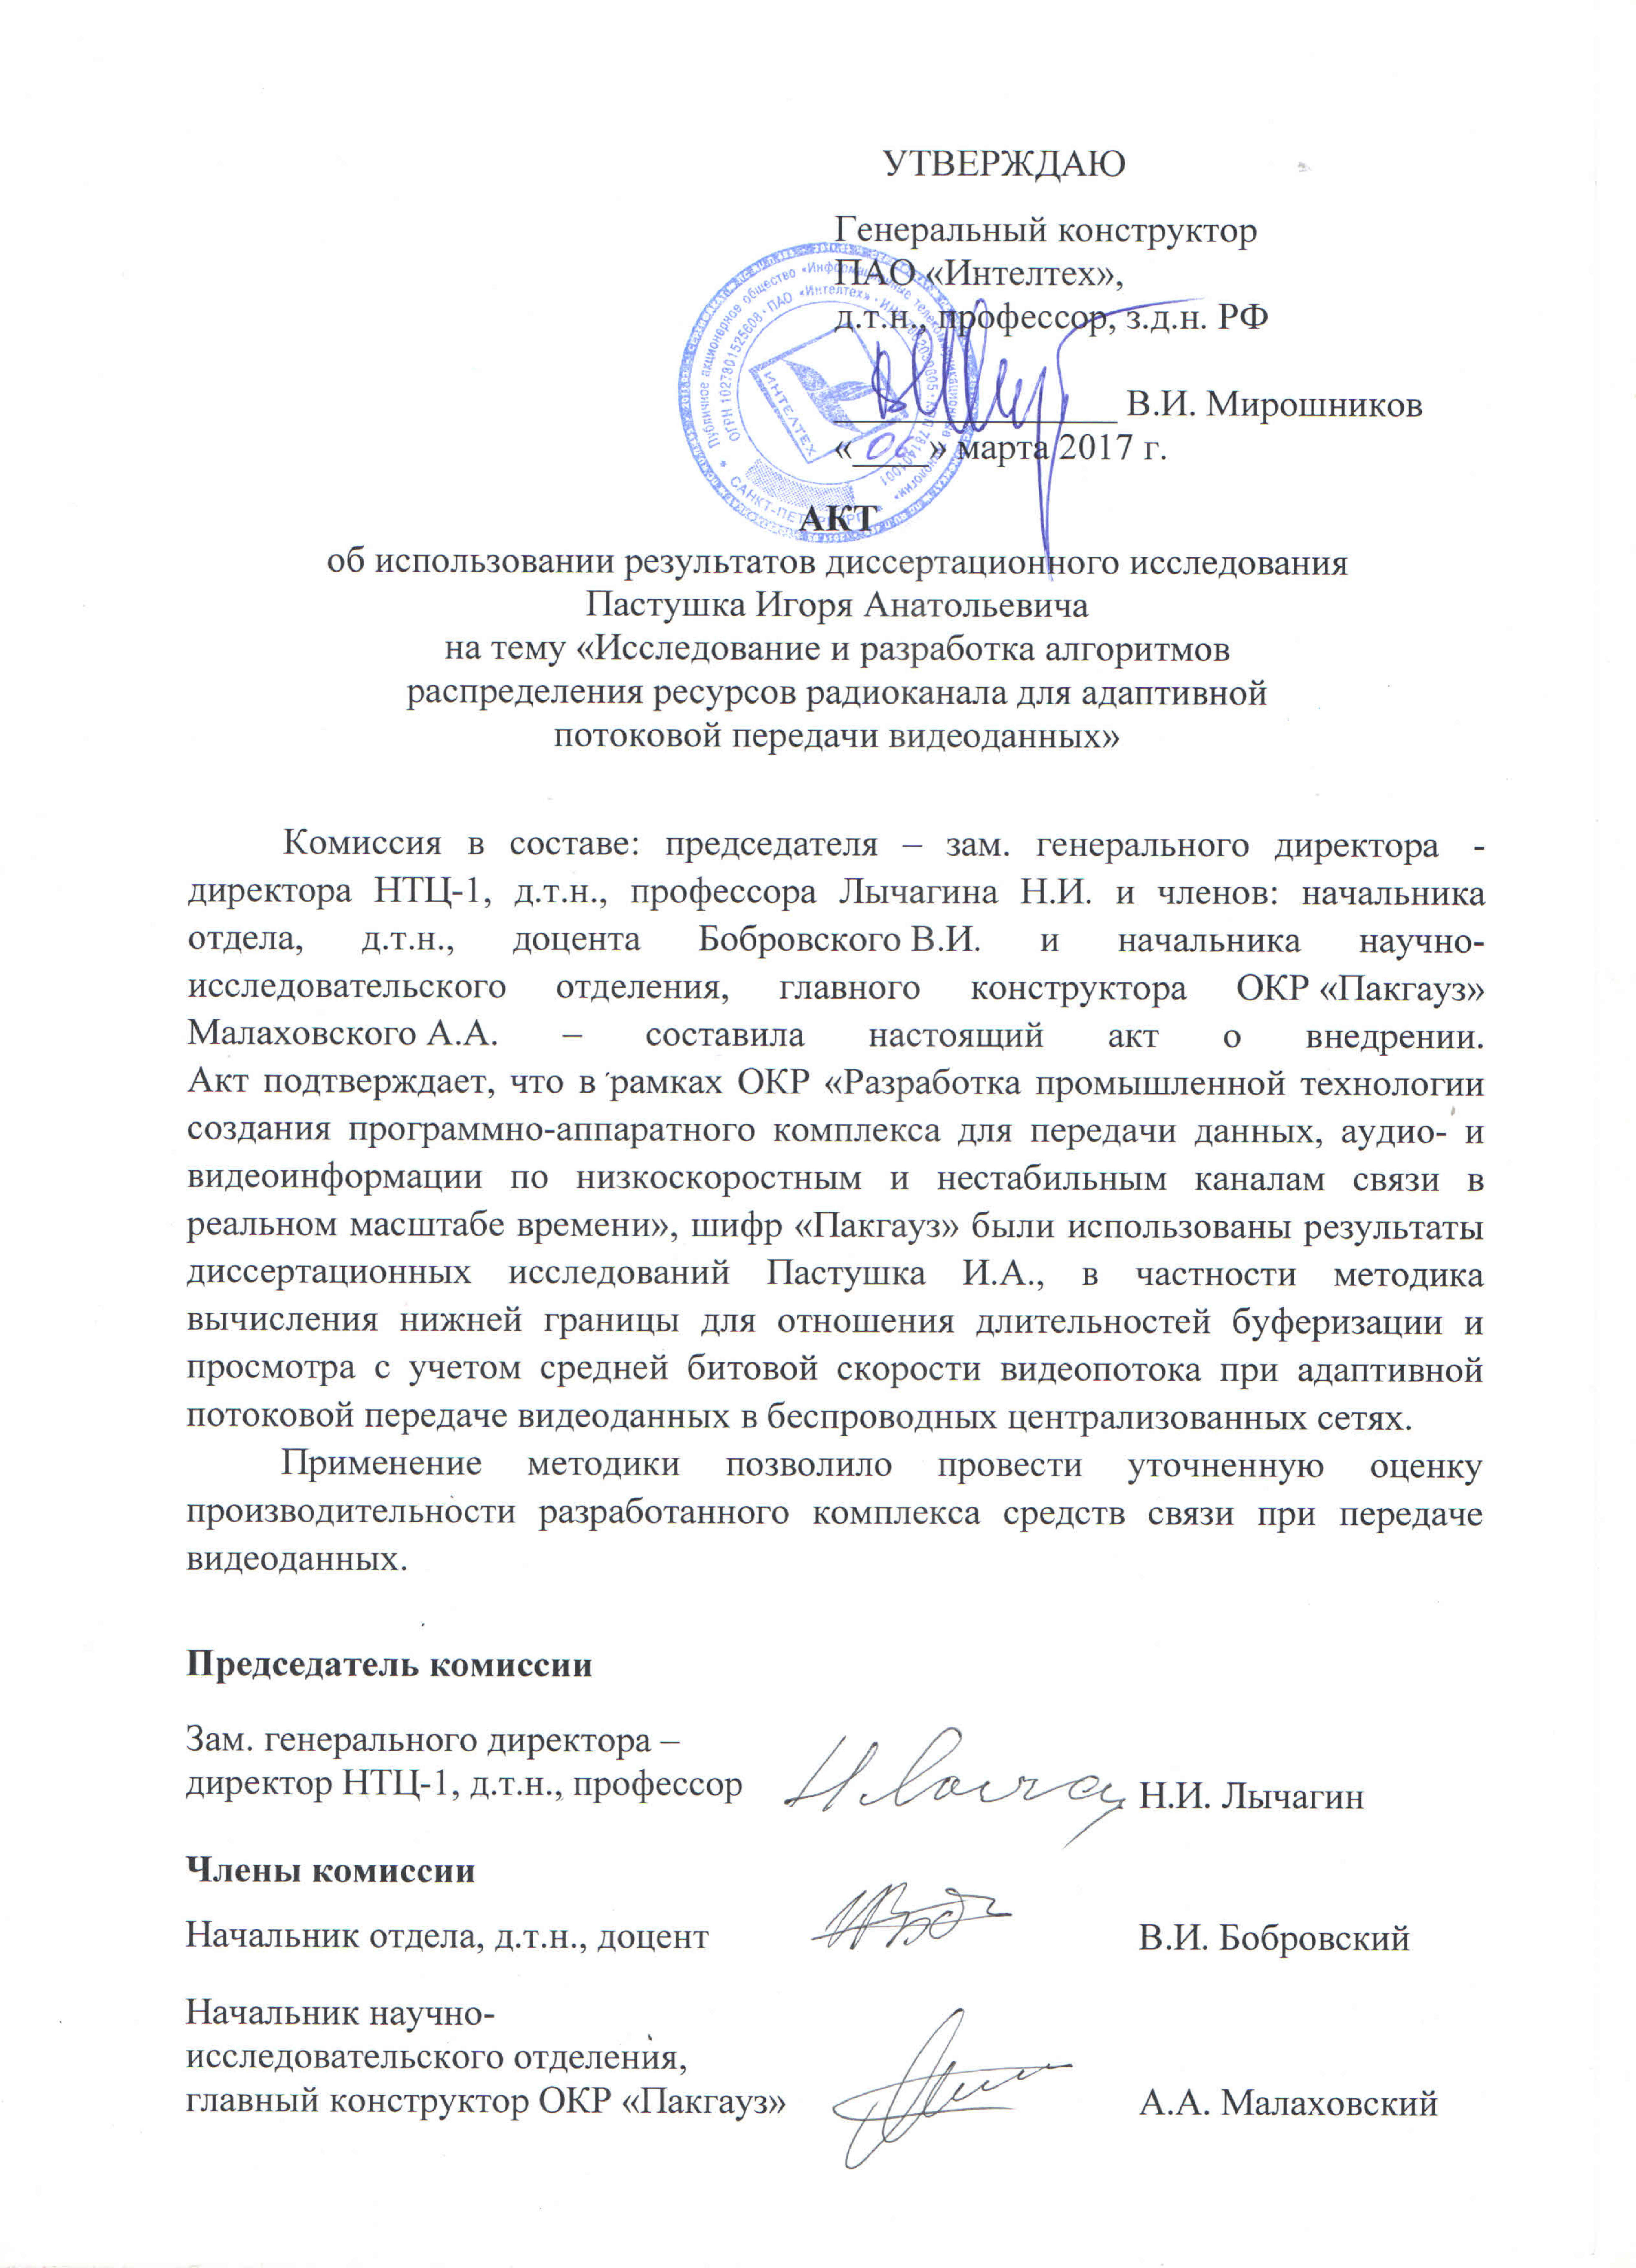
\includepdf[width=1.2\textwidth,height=0.7\textheight]{appendix/Inteltech.pdf}
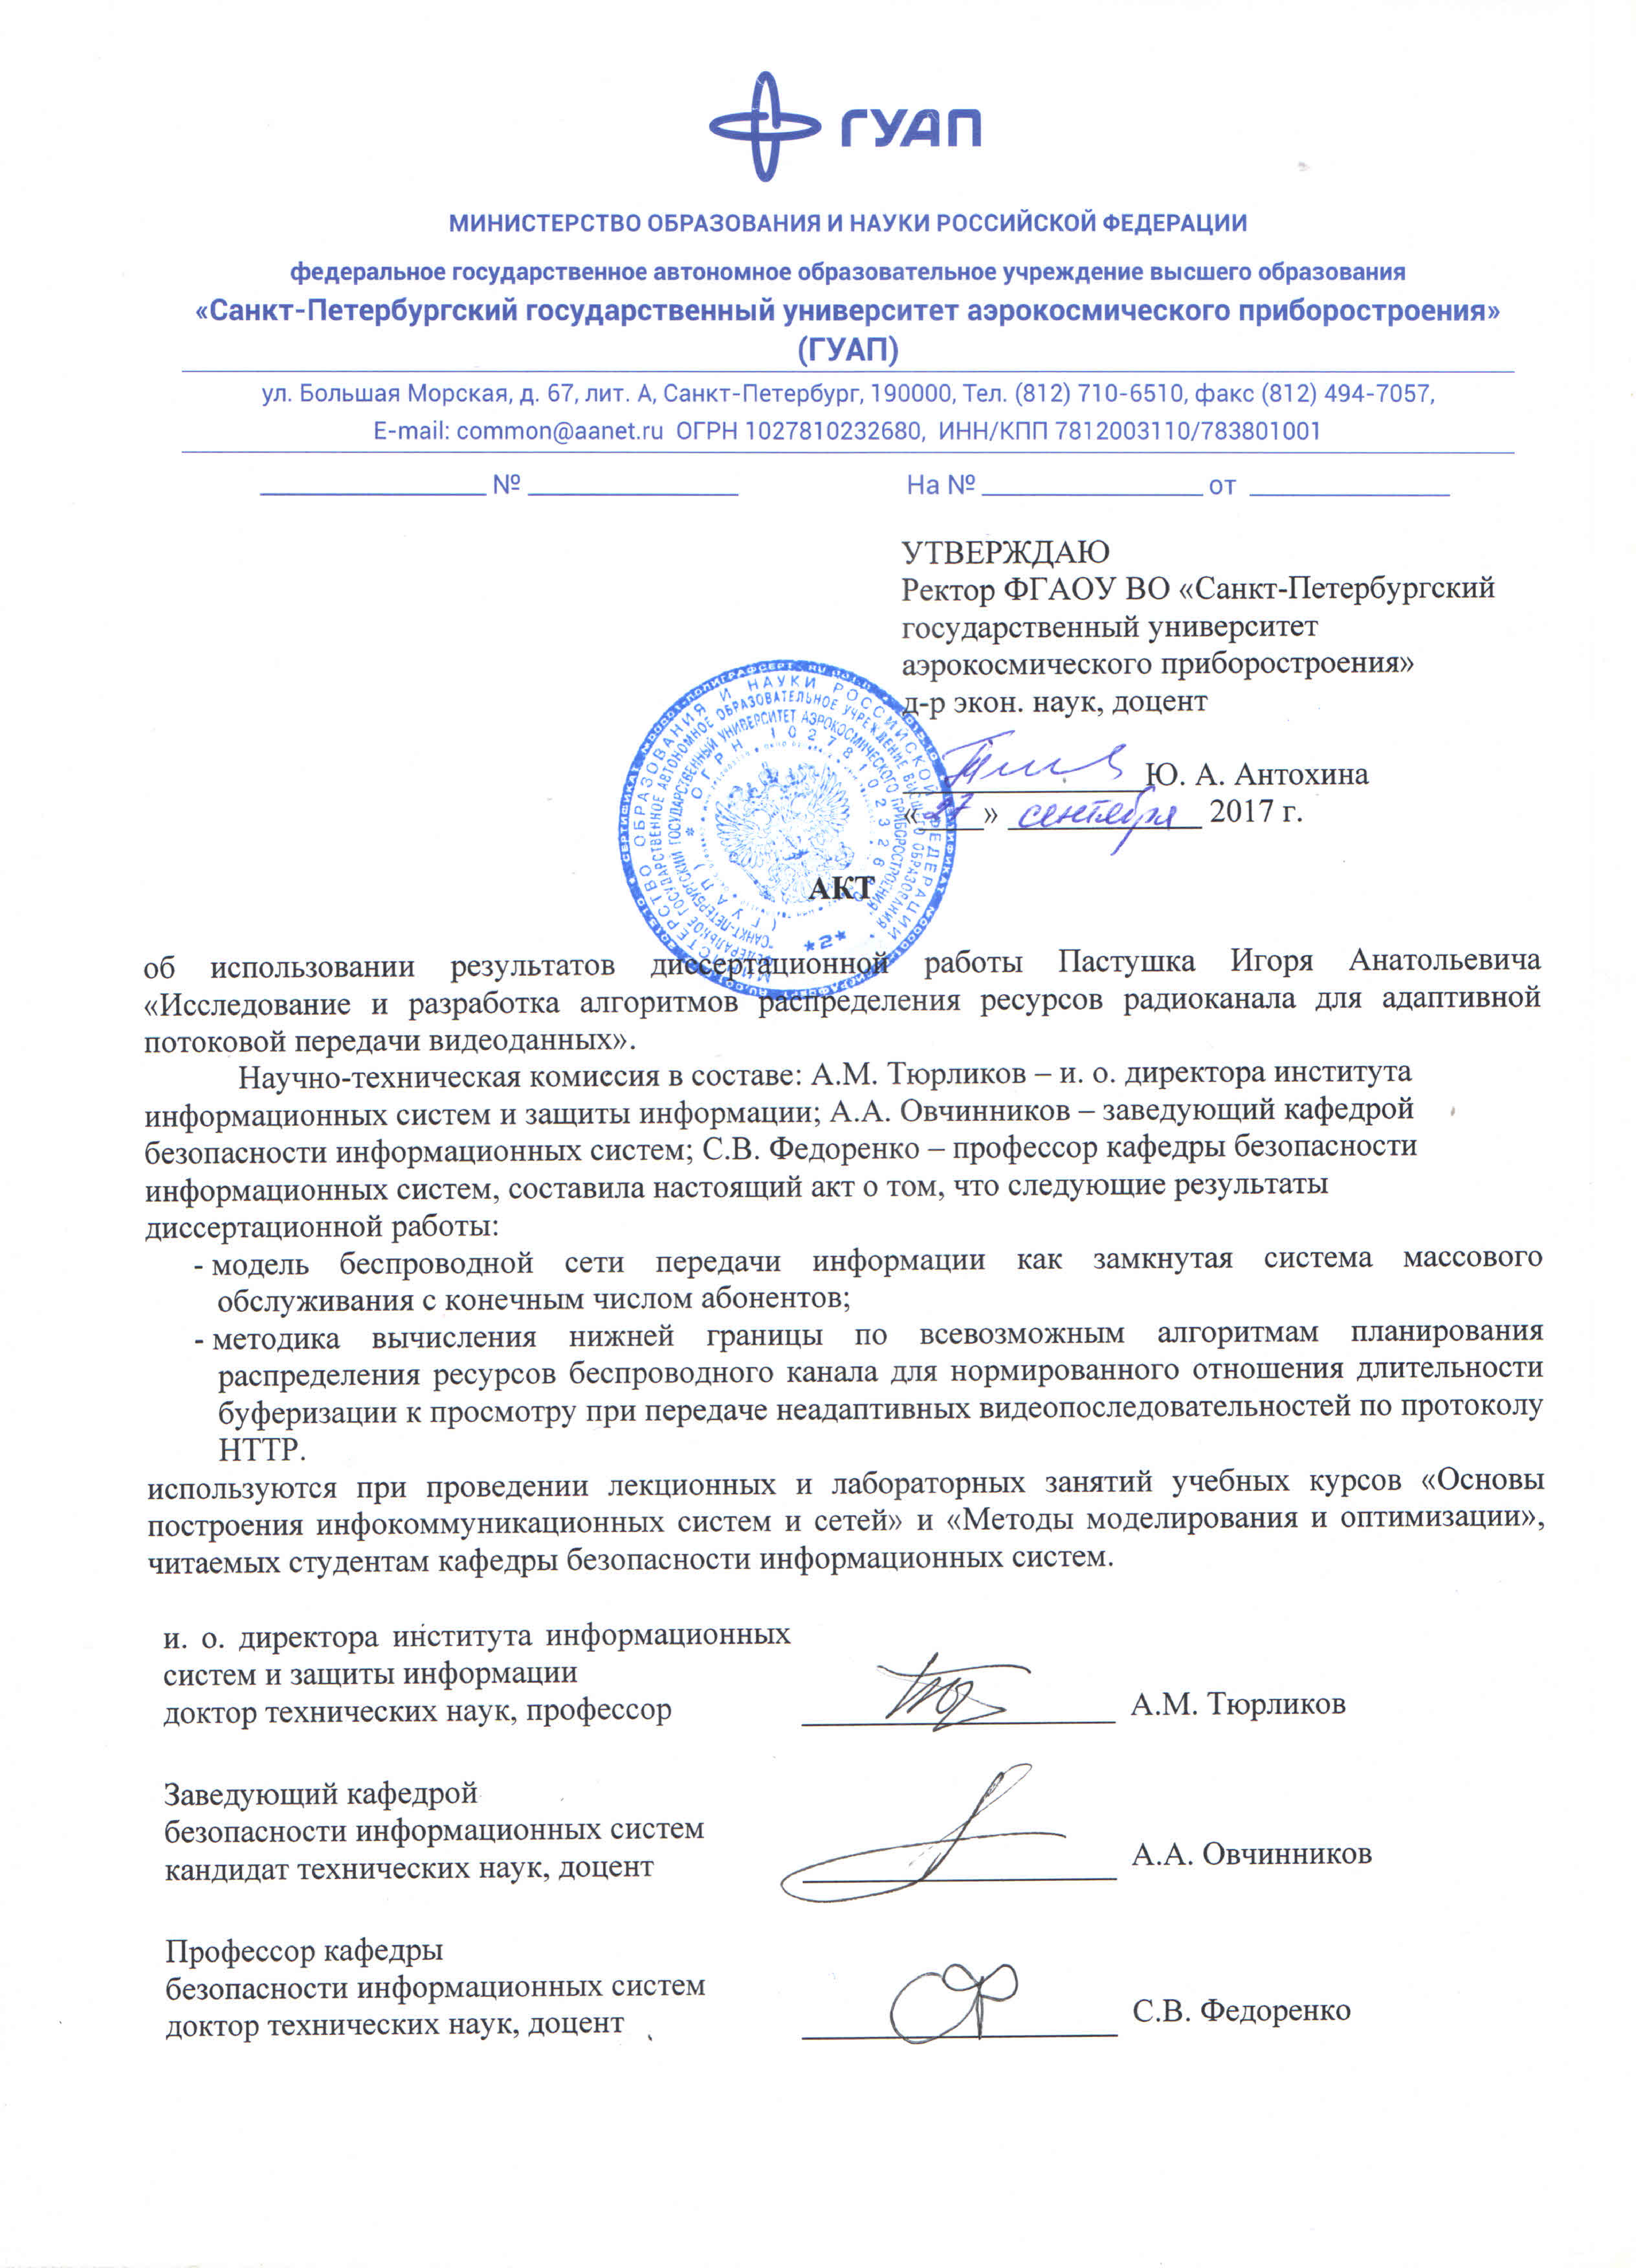
\includepdf{appendix/Act51.pdf}

\includepdf{appendix/Act52.pdf}
%\chapter{Примеры вставки листингов программного кода} \label{AppendixA}
%
%Для крупных листингов есть два способа. Первый красивый, но в нём могут быть проблемы с поддержкой кириллицы (у вас может встречаться в комментариях и
%печатаемых сообщениях), он представлен на листинге~\ref{list:hwbeauty}.
%%\renewcommand\FBbskip{-20pt} % если хотим притянуть что-то к плавающему окружению из floatrow
%\begin{ListingEnv}[H]% буква H означает Here, ставим здесь,
%    % элементы, которые нежелательно разрывать обычно не ставят
%    % посреди страницы: вместо H используется t (top, сверху страницы),
%    % или b (bottom) или p (page, на отдельной странице)
%%    \captionsetup{format=tablenocaption}% должен стоять до самого caption
%%    \thisfloatsetup{\capposition=top}%
%    \caption{Программа “Hello, world” на \protect\cpp}
%    % далее метка для ссылки:
%    \label{list:hwbeauty}
%    % окружение учитывает пробелы и табляции и приеняет их в сответсвии с настройкми
%    \begin{lstlisting}[language={[ISO]C++}]
%	#include <iostream>
%	using namespace std;
%
%	int main() //кириллица в комментариях при xelatex и lualatex имеет проблемы с пробелами
%	{
%		cout << "Hello, world" << endl; //latin letters in commentaries
%		system("pause");
%		return 0;
%	}
%    \end{lstlisting}
%\end{ListingEnv}%
%Второй не такой красивый, но без ограничений (см.~листинг~\ref{list:hwplain}).
%\begin{ListingEnv}[H]
%    \begin{Verb}
%
%        #include <iostream>
%        using namespace std;
%
%        int main() //кириллица в комментариях
%        {
%            cout << "Привет, мир" << endl;
%        }
%    \end{Verb}
%    \caption{Программа “Hello, world” без подсветки}
%    \label{list:hwplain}
%\end{ListingEnv}
%
%Можно использовать первый для вставки небольших фрагментов
%внутри текста, а второй для вставки полного
%кода в приложении, если таковое имеется.
%
%Если нужно вставить совсем короткий пример кода (одна или две строки), то выделение  линейками и нумерация может смотреться чересчур громоздко. В таких случаях можно использовать окружения \texttt{lstlisting} или \texttt{Verb} без \texttt{ListingEnv}. Приведём такой пример с указанием языка программирования, отличного от заданного по умолчанию:
%\begin{lstlisting}[language=Haskell]
%fibs = 0 : 1 : zipWith (+) fibs (tail fibs)
%\end{lstlisting}
%Такое решение~--- со вставкой нумерованных листингов покрупнее
%и вставок без выделения для маленьких фрагментов~--- выбрано,
%например, в книге Эндрю Таненбаума и Тодда Остина по архитектуре
%%компьютера~\autocite{TanAus2013} (см.~рис.~\ref{fig:tan-aus}).
%
%Наконец, для оформления идентификаторов внутри строк
%(функция \lstinline{main} и тому подобное) используется
%\texttt{lstinline} или, самое простое, моноширинный текст
%(\texttt{\textbackslash texttt}).
%
%
%Пример~\ref{list:internal3}, иллюстрирующий подключение переопределённого языка. Может быть полезным, если подсветка кода работает криво. Без дополнительного окружения, с подписью и ссылкой, реализованной встроенным средством.
%\begin{lstlisting}[language={Renhanced},caption={Пример листинга c подписью собственными средствами},label={list:internal3}]
%## Caching the Inverse of a Matrix
%
%## Matrix inversion is usually a costly computation and there may be some
%## benefit to caching the inverse of a matrix rather than compute it repeatedly
%## This is a pair of functions that cache the inverse of a matrix.
%
%## makeCacheMatrix creates a special "matrix" object that can cache its inverse
%
%makeCacheMatrix <- function(x = matrix()) {#кириллица в комментариях при xelatex b lualatex имеет проблемы с пробелами
%    i <- NULL
%    set <- function(y) {
%        x <<- y
%        i <<- NULL
%    }
%    get <- function() x
%    setSolved <- function(solve) i <<- solve
%    getSolved <- function() i
%    list(set = set, get = get,
%    setSolved = setSolved,
%    getSolved = getSolved)
%
%}
%
%
%## cacheSolve computes the inverse of the special "matrix" returned by
%## makeCacheMatrix above. If the inverse has already been calculated (and the
%## matrix has not changed), then the cachesolve should retrieve the inverse from
%## the cache.
%
%cacheSolve <- function(x, ...) {
%    ## Return a matrix that is the inverse of 'x'
%    i <- x$getSolved()
%    if(!is.null(i)) {
%        message("getting cached data")
%        return(i)
%    }
%    data <- x$get()
%    i <- solve(data, ...)
%    x$setSolved(i)
%    i
%}
%\end{lstlisting}
%
%Листинг~\ref{list:external1} подгружается из внешнего файла. Приходится загружать без окружения дополнительного. Иначе по страницам не переносится.
%    \lstinputlisting[lastline=78,language={R},caption={Листинг из внешнего файла},label={list:external1}]{./listings/run_analysis.R}
%
%
%
%
%
%
%\chapter{Очень длинное название второго приложения, в котором продемонстрирована работа с длинными таблицами} \label{AppendixB}
%
% \section{Подраздел приложения}\label{AppendixB1}
%Вот размещается длинная таблица:
%\fontsize{10pt}{10pt}\selectfont
%\begin{longtable}[c]{|l|c|l|l|}
%% \caption{Описание входных файлов модели}\label{Namelists}
%%\\
% \hline
% %\multicolumn{4}{|c|}{\textbf{Файл puma\_namelist}}        \\ \hline
% Параметр & Умолч. & Тип & Описание               \\ \hline
%                                              \endfirsthead   \hline
% \multicolumn{4}{|c|}{\small\slshape (продолжение)}        \\ \hline
% Параметр & Умолч. & Тип & Описание               \\ \hline
%                                              \endhead        \hline
% \multicolumn{4}{|r|}{\small\slshape продолжение следует}  \\ \hline
%                                              \endfoot        \hline
%                                              \endlastfoot
% \multicolumn{4}{|l|}{\&INP}        \\ \hline
% kick & 1 & int & 0: инициализация без шума ($p_s = const$) \\
%      &   &     & 1: генерация белого шума                  \\
%      &   &     & 2: генерация белого шума симметрично относительно \\
%  & & & экватора    \\
% mars & 0 & int & 1: инициализация модели для планеты Марс     \\
% kick & 1 & int & 0: инициализация без шума ($p_s = const$) \\
%      &   &     & 1: генерация белого шума                  \\
%      &   &     & 2: генерация белого шума симметрично относительно \\
%  & & & экватора    \\
% mars & 0 & int & 1: инициализация модели для планеты Марс     \\
%kick & 1 & int & 0: инициализация без шума ($p_s = const$) \\
%      &   &     & 1: генерация белого шума                  \\
%      &   &     & 2: генерация белого шума симметрично относительно \\
%  & & & экватора    \\
% mars & 0 & int & 1: инициализация модели для планеты Марс     \\
%kick & 1 & int & 0: инициализация без шума ($p_s = const$) \\
%      &   &     & 1: генерация белого шума                  \\
%      &   &     & 2: генерация белого шума симметрично относительно \\
%  & & & экватора    \\
% mars & 0 & int & 1: инициализация модели для планеты Марс     \\
%kick & 1 & int & 0: инициализация без шума ($p_s = const$) \\
%      &   &     & 1: генерация белого шума                  \\
%      &   &     & 2: генерация белого шума симметрично относительно \\
%  & & & экватора    \\
% mars & 0 & int & 1: инициализация модели для планеты Марс     \\
%kick & 1 & int & 0: инициализация без шума ($p_s = const$) \\
%      &   &     & 1: генерация белого шума                  \\
%      &   &     & 2: генерация белого шума симметрично относительно \\
%  & & & экватора    \\
% mars & 0 & int & 1: инициализация модели для планеты Марс     \\
%kick & 1 & int & 0: инициализация без шума ($p_s = const$) \\
%      &   &     & 1: генерация белого шума                  \\
%      &   &     & 2: генерация белого шума симметрично относительно \\
%  & & & экватора    \\
% mars & 0 & int & 1: инициализация модели для планеты Марс     \\
%kick & 1 & int & 0: инициализация без шума ($p_s = const$) \\
%      &   &     & 1: генерация белого шума                  \\
%      &   &     & 2: генерация белого шума симметрично относительно \\
%  & & & экватора    \\
% mars & 0 & int & 1: инициализация модели для планеты Марс     \\
%kick & 1 & int & 0: инициализация без шума ($p_s = const$) \\
%      &   &     & 1: генерация белого шума                  \\
%      &   &     & 2: генерация белого шума симметрично относительно \\
%  & & & экватора    \\
% mars & 0 & int & 1: инициализация модели для планеты Марс     \\
%kick & 1 & int & 0: инициализация без шума ($p_s = const$) \\
%      &   &     & 1: генерация белого шума                  \\
%      &   &     & 2: генерация белого шума симметрично относительно \\
%  & & & экватора    \\
% mars & 0 & int & 1: инициализация модели для планеты Марс     \\
%kick & 1 & int & 0: инициализация без шума ($p_s = const$) \\
%      &   &     & 1: генерация белого шума                  \\
%      &   &     & 2: генерация белого шума симметрично относительно \\
%  & & & экватора    \\
% mars & 0 & int & 1: инициализация модели для планеты Марс     \\
%kick & 1 & int & 0: инициализация без шума ($p_s = const$) \\
%      &   &     & 1: генерация белого шума                  \\
%      &   &     & 2: генерация белого шума симметрично относительно \\
%  & & & экватора    \\
% mars & 0 & int & 1: инициализация модели для планеты Марс     \\
%kick & 1 & int & 0: инициализация без шума ($p_s = const$) \\
%      &   &     & 1: генерация белого шума                  \\
%      &   &     & 2: генерация белого шума симметрично относительно \\
%  & & & экватора    \\
% mars & 0 & int & 1: инициализация модели для планеты Марс     \\
%kick & 1 & int & 0: инициализация без шума ($p_s = const$) \\
%      &   &     & 1: генерация белого шума                  \\
%      &   &     & 2: генерация белого шума симметрично относительно \\
%  & & & экватора    \\
% mars & 0 & int & 1: инициализация модели для планеты Марс     \\
%kick & 1 & int & 0: инициализация без шума ($p_s = const$) \\
%      &   &     & 1: генерация белого шума                  \\
%      &   &     & 2: генерация белого шума симметрично относительно \\
%  & & & экватора    \\
% mars & 0 & int & 1: инициализация модели для планеты Марс     \\
% \hline
%  %& & & $\:$ \\
% \multicolumn{4}{|l|}{\&SURFPAR}        \\ \hline
%kick & 1 & int & 0: инициализация без шума ($p_s = const$) \\
%      &   &     & 1: генерация белого шума                  \\
%      &   &     & 2: генерация белого шума симметрично относительно \\
%  & & & экватора    \\
% mars & 0 & int & 1: инициализация модели для планеты Марс     \\
%kick & 1 & int & 0: инициализация без шума ($p_s = const$) \\
%      &   &     & 1: генерация белого шума                  \\
%      &   &     & 2: генерация белого шума симметрично относительно \\
%  & & & экватора    \\
% mars & 0 & int & 1: инициализация модели для планеты Марс     \\
%kick & 1 & int & 0: инициализация без шума ($p_s = const$) \\
%      &   &     & 1: генерация белого шума                  \\
%      &   &     & 2: генерация белого шума симметрично относительно \\
%  & & & экватора    \\
% mars & 0 & int & 1: инициализация модели для планеты Марс     \\
%kick & 1 & int & 0: инициализация без шума ($p_s = const$) \\
%      &   &     & 1: генерация белого шума                  \\
%      &   &     & 2: генерация белого шума симметрично относительно \\
%  & & & экватора    \\
% mars & 0 & int & 1: инициализация модели для планеты Марс     \\
%kick & 1 & int & 0: инициализация без шума ($p_s = const$) \\
%      &   &     & 1: генерация белого шума                  \\
%      &   &     & 2: генерация белого шума симметрично относительно \\
%  & & & экватора    \\
% mars & 0 & int & 1: инициализация модели для планеты Марс     \\
%kick & 1 & int & 0: инициализация без шума ($p_s = const$) \\
%      &   &     & 1: генерация белого шума                  \\
%      &   &     & 2: генерация белого шума симметрично относительно \\
%  & & & экватора    \\
% mars & 0 & int & 1: инициализация модели для планеты Марс     \\
%kick & 1 & int & 0: инициализация без шума ($p_s = const$) \\
%      &   &     & 1: генерация белого шума                  \\
%      &   &     & 2: генерация белого шума симметрично относительно \\
%  & & & экватора    \\
% mars & 0 & int & 1: инициализация модели для планеты Марс     \\
%kick & 1 & int & 0: инициализация без шума ($p_s = const$) \\
%      &   &     & 1: генерация белого шума                  \\
%      &   &     & 2: генерация белого шума симметрично относительно \\
%  & & & экватора    \\
% mars & 0 & int & 1: инициализация модели для планеты Марс     \\
%kick & 1 & int & 0: инициализация без шума ($p_s = const$) \\
%      &   &     & 1: генерация белого шума                  \\
%      &   &     & 2: генерация белого шума симметрично относительно \\
%  & & & экватора    \\
% mars & 0 & int & 1: инициализация модели для планеты Марс     \\
% \hline
%\end{longtable}
%
%\normalsize% возвращаем шрифт к нормальному
%\section{Ещё один подраздел приложения} \label{AppendixB2}
%
%Нужно больше подразделов приложения!
%
%Пример длинной таблицы с записью продолжения по ГОСТ 2.105
%
%    \centering
%	\small
%    \begin{longtable}[c]{|l|c|l|l|}
%	\caption{Наименование таблицы средней длины}%
%    \label{tbl:test5}% label всегда желательно идти после caption
%    \\
%    \hline
%     %\multicolumn{4}{|c|}{\textbf{Файл puma\_namelist}}        \\ \hline
%     Параметр & Умолч. & Тип & Описание               \\ \hline
%                                                  \endfirsthead
%%     \multicolumn{4}{|c|}{\small\slshape (продолжение)}        \\ \hline
% \captionsetup{format=tablenocaption,labelformat=continued}% должен стоять до самого caption
% \caption[]{} \\
%    \hline
%     Параметр & Умолч. & Тип & Описание               \\ \hline
%                                                  \endhead        \hline
%%     \multicolumn{4}{|r|}{\small\slshape продолжение следует}  \\
%%\hline
%                                                  \endfoot        \hline
%                                                  \endlastfoot
%     \multicolumn{4}{|l|}{\&INP}        \\ \hline
%     kick & 1 & int & 0: инициализация без шума ($p_s = const$) \\
%          &   &     & 1: генерация белого шума                  \\
%          &   &     & 2: генерация белого шума симметрично относительно \\
%      & & & экватора    \\
%     mars & 0 & int & 1: инициализация модели для планеты Марс     \\
%     kick & 1 & int & 0: инициализация без шума ($p_s = const$) \\
%          &   &     & 1: генерация белого шума                  \\
%          &   &     & 2: генерация белого шума симметрично относительно \\
%      & & & экватора    \\
%     mars & 0 & int & 1: инициализация модели для планеты Марс     \\
%    kick & 1 & int & 0: инициализация без шума ($p_s = const$) \\
%          &   &     & 1: генерация белого шума                  \\
%          &   &     & 2: генерация белого шума симметрично относительно \\
%      & & & экватора    \\
%     mars & 0 & int & 1: инициализация модели для планеты Марс     \\
%    kick & 1 & int & 0: инициализация без шума ($p_s = const$) \\
%          &   &     & 1: генерация белого шума                  \\
%          &   &     & 2: генерация белого шума симметрично относительно \\
%      & & & экватора    \\
%     mars & 0 & int & 1: инициализация модели для планеты Марс     \\
%    kick & 1 & int & 0: инициализация без шума ($p_s = const$) \\
%          &   &     & 1: генерация белого шума                  \\
%          &   &     & 2: генерация белого шума симметрично относительно \\
%      & & & экватора    \\
%     mars & 0 & int & 1: инициализация модели для планеты Марс     \\
%    kick & 1 & int & 0: инициализация без шума ($p_s = const$) \\
%          &   &     & 1: генерация белого шума                  \\
%          &   &     & 2: генерация белого шума симметрично относительно \\
%      & & & экватора    \\
%     mars & 0 & int & 1: инициализация модели для планеты Марс     \\
%    kick & 1 & int & 0: инициализация без шума ($p_s = const$) \\
%          &   &     & 1: генерация белого шума                  \\
%          &   &     & 2: генерация белого шума симметрично относительно \\
%      & & & экватора    \\
%     mars & 0 & int & 1: инициализация модели для планеты Марс     \\
%    kick & 1 & int & 0: инициализация без шума ($p_s = const$) \\
%          &   &     & 1: генерация белого шума                  \\
%          &   &     & 2: генерация белого шума симметрично относительно \\
%      & & & экватора    \\
%     mars & 0 & int & 1: инициализация модели для планеты Марс     \\
%    kick & 1 & int & 0: инициализация без шума ($p_s = const$) \\
%          &   &     & 1: генерация белого шума                  \\
%          &   &     & 2: генерация белого шума симметрично относительно \\
%      & & & экватора    \\
%     mars & 0 & int & 1: инициализация модели для планеты Марс     \\
%    kick & 1 & int & 0: инициализация без шума ($p_s = const$) \\
%          &   &     & 1: генерация белого шума                  \\
%          &   &     & 2: генерация белого шума симметрично относительно \\
%      & & & экватора    \\
%     mars & 0 & int & 1: инициализация модели для планеты Марс     \\
%    kick & 1 & int & 0: инициализация без шума ($p_s = const$) \\
%          &   &     & 1: генерация белого шума                  \\
%          &   &     & 2: генерация белого шума симметрично относительно \\
%      & & & экватора    \\
%     mars & 0 & int & 1: инициализация модели для планеты Марс     \\
%    kick & 1 & int & 0: инициализация без шума ($p_s = const$) \\
%          &   &     & 1: генерация белого шума                  \\
%          &   &     & 2: генерация белого шума симметрично относительно \\
%      & & & экватора    \\
%     mars & 0 & int & 1: инициализация модели для планеты Марс     \\
%    kick & 1 & int & 0: инициализация без шума ($p_s = const$) \\
%          &   &     & 1: генерация белого шума                  \\
%          &   &     & 2: генерация белого шума симметрично относительно \\
%      & & & экватора    \\
%     mars & 0 & int & 1: инициализация модели для планеты Марс     \\
%    kick & 1 & int & 0: инициализация без шума ($p_s = const$) \\
%          &   &     & 1: генерация белого шума                  \\
%          &   &     & 2: генерация белого шума симметрично относительно \\
%      & & & экватора    \\
%     mars & 0 & int & 1: инициализация модели для планеты Марс     \\
%    kick & 1 & int & 0: инициализация без шума ($p_s = const$) \\
%          &   &     & 1: генерация белого шума                  \\
%          &   &     & 2: генерация белого шума симметрично относительно \\
%      & & & экватора    \\
%     mars & 0 & int & 1: инициализация модели для планеты Марс     \\
%     \hline
%      %& & & $\:$ \\
%     \multicolumn{4}{|l|}{\&SURFPAR}        \\ \hline
%    kick & 1 & int & 0: инициализация без шума ($p_s = const$) \\
%          &   &     & 1: генерация белого шума                  \\
%          &   &     & 2: генерация белого шума симметрично относительно \\
%      & & & экватора    \\
%     mars & 0 & int & 1: инициализация модели для планеты Марс     \\
%    kick & 1 & int & 0: инициализация без шума ($p_s = const$) \\
%          &   &     & 1: генерация белого шума                  \\
%          &   &     & 2: генерация белого шума симметрично относительно \\
%      & & & экватора    \\
%     mars & 0 & int & 1: инициализация модели для планеты Марс     \\
%    kick & 1 & int & 0: инициализация без шума ($p_s = const$) \\
%          &   &     & 1: генерация белого шума                  \\
%          &   &     & 2: генерация белого шума симметрично относительно \\
%      & & & экватора    \\
%     mars & 0 & int & 1: инициализация модели для планеты Марс     \\
%    kick & 1 & int & 0: инициализация без шума ($p_s = const$) \\
%          &   &     & 1: генерация белого шума                  \\
%          &   &     & 2: генерация белого шума симметрично относительно \\
%      & & & экватора    \\
%     mars & 0 & int & 1: инициализация модели для планеты Марс     \\
%    kick & 1 & int & 0: инициализация без шума ($p_s = const$) \\
%          &   &     & 1: генерация белого шума                  \\
%          &   &     & 2: генерация белого шума симметрично относительно \\
%      & & & экватора    \\
%     mars & 0 & int & 1: инициализация модели для планеты Марс     \\
%    kick & 1 & int & 0: инициализация без шума ($p_s = const$) \\
%          &   &     & 1: генерация белого шума                  \\
%          &   &     & 2: генерация белого шума симметрично относительно \\
%      & & & экватора    \\
%     mars & 0 & int & 1: инициализация модели для планеты Марс     \\
%    kick & 1 & int & 0: инициализация без шума ($p_s = const$) \\
%          &   &     & 1: генерация белого шума                  \\
%          &   &     & 2: генерация белого шума симметрично относительно \\
%      & & & экватора    \\
%     mars & 0 & int & 1: инициализация модели для планеты Марс     \\
%    kick & 1 & int & 0: инициализация без шума ($p_s = const$) \\
%          &   &     & 1: генерация белого шума                  \\
%          &   &     & 2: генерация белого шума симметрично относительно \\
%      & & & экватора    \\
%     mars & 0 & int & 1: инициализация модели для планеты Марс     \\
%    kick & 1 & int & 0: инициализация без шума ($p_s = const$) \\
%          &   &     & 1: генерация белого шума                  \\
%          &   &     & 2: генерация белого шума симметрично относительно \\
%      & & & экватора    \\
%     mars & 0 & int & 1: инициализация модели для планеты Марс     \\
%     \hline
%    \end{longtable}
%\normalsize% возвращаем шрифт к нормальному
%\section{Очередной подраздел приложения} \label{AppendixB3}
%
%Нужно больше подразделов приложения!
%
%\section{И ещё один подраздел приложения} \label{AppendixB4}
%
%Нужно больше подразделов приложения!

